\chapter{The $\mathrm{Z}$ boson transverse momentum correction}

%Talk mainly about the PTZ stuff here, can briefly mentioned the ID and reco SF stuff. Mention JER and JES here too.
Dedicated corrections are applied to the dielectron \pt spectrum in simulated Drell-Yan events in order to improve the agreement between simulation and data. These aim to correct differences with respect to data at low \pt, where the emission of soft gluons and associated re-summation effects are not accounted for in simulation~\cite{dy_pt_mismodelling}.
This leads to a softer \pt spectrum in simulation, compared to data. %QCD calculations are tricky for low Q^2 interactions as terms are large and diverge (coupling increases as energy decreases)!
To correct for this effect, a simple reweighting of the simulation to data is performed. This correction acts only to improve the performance of the classifiers used in the event categorisation (that are trained on DY events), rather than to correct background models, which are taken directly from data. The reweighting is derived in bins of dielectron \pt in the analysis control region around the Z boson mass. Scale factors are derived in a binning scheme that roughly evolves with the yield in the control region; the bin widths are 1.6~GeV, 4~GeV, and 5~GeV for the regions $0 < p_{T,ee} \leq 40$~GeV, $40< p_{T,ee} \leq 80$~GeV, $80< p_{T,ee} \leq 180$~GeV respectively. No correction is derived for events with $p_{T,ee} > 180$~GeV, since the relative statistical uncertainty on the simulation is large. Corrections are also derived separately for each year of data taking, to account for potential per-year differences. To illustrate the impact of this correction, Figure \ref{fig:ggH_ptee_reweighting} shows the dielectron \pt distribution in the signal region, before and after the \pt reweighting is applied. Good agreement is observed between the corrected simulation and data, particularly in the low \pt regime. A doubly-differential reweighting was also attempted by further partitioning events into bins of jet multiplicity (0-jet, 1-jet, and $\geq2$-jets). The additional binning does not significantly improve the agreement between simulation and data; it is therefore sufficient to reweight DY samples in bins of $p_{T,ee}$ only.

\begin{figure}[htbp!]
\centering
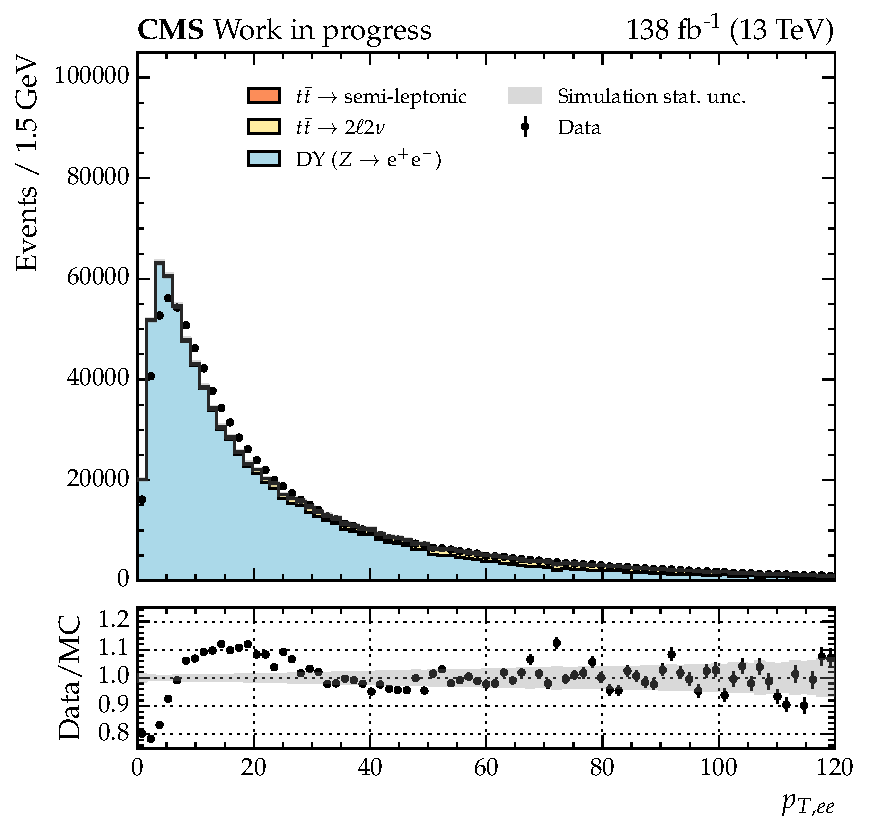
\includegraphics[width =0.46\linewidth]{Figures/Hee/simulationCorrections/DY/ggH_BDT_dielectronPt.pdf}\hfill%
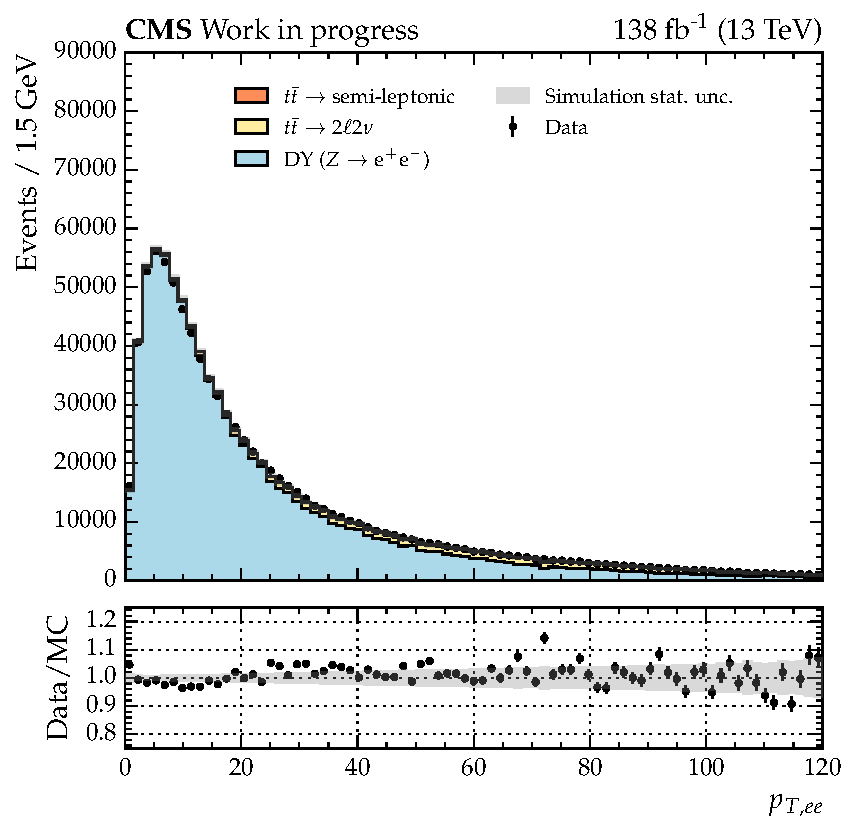
\includegraphics[width =0.46\linewidth]{Figures/Hee/simulationCorrections/DY/ggH_BDT_pt_reweighted_dielectronPt.pdf}\hfill%
\caption[The dielectron transverse momentum distribution for simulated background events, corrected by scale factors derived in the \Hee control region.]{Distributions of $p_{T,ee}$ for simulated Drell-Yan events, additional \ttbar backgrounds, and data in the signal region. The statistical uncertainty on the total background yield is shown in the grey shaded band. Left: nominal $p_{T,ee}$ distribution with no correction applied. Right: $p_{T,ee}$ distribution where Drell-Yan simulation is corrected by scale factors derived in a control region around the Z boson mass. A significant improvement in agreement between data and simulation is observed following these corrections, particularly in the low $p_{T,ee}$ regime.}
\label{fig:ggH_ptee_reweighting}
\end{figure}